\section{Parallelisierung}

\begin{frame}
\frametitle{Parallelisierung} 
	\begin{itemize}[<+->]
		\item OpenMP
		\item \lstinputlisting{./parallel_for.c}
		\item Ein gemeinsamer Speicher
		\item Gauss-Seidel und OpemMP
	\end{itemize}
\end{frame}

\begin{frame}
	\centering
	Nach dem ersten Schritt mit 32 Threads:
	
	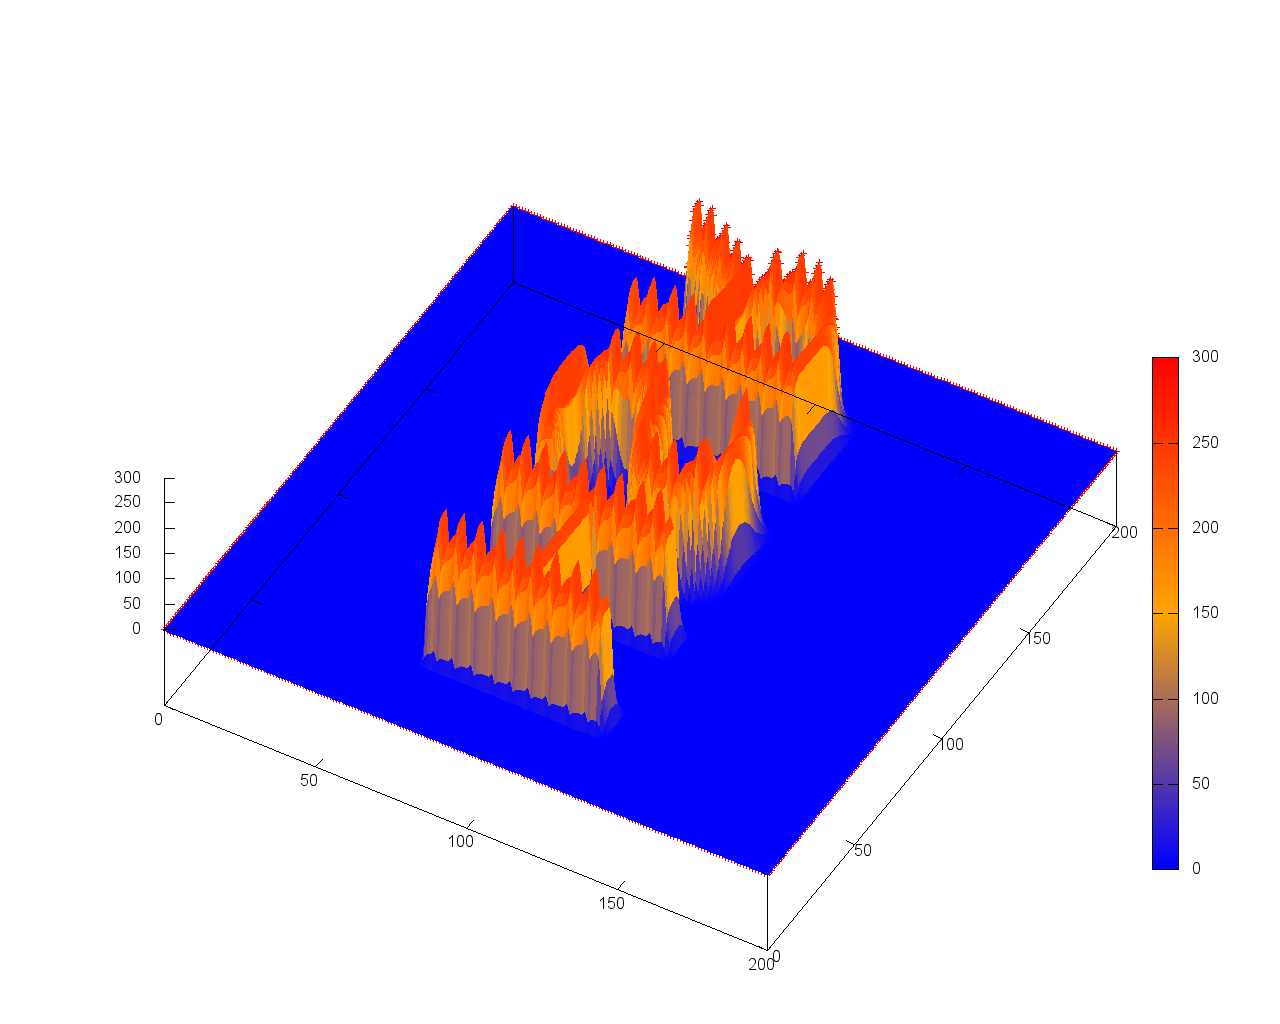
\includegraphics[width = 10cm]{../skript/images/step001}
\end{frame}
